\section{ダイレクトティーチング}
\label{sec:direct_teaching}

\subsection{実験内容}
\subsubsection{手順}
ダイレクトティーチングとは,手動で手先を動かし,2軸ロボットにその動きを再現させることである.ダイレクトティーチングを行うためには,以下のステップを実行すればよい.

\underline{\textbf{ステップ 1}}\quad 
手先位置 $P_3$ が所望の軌道に沿うように手先を手で動かし,関節角 $\theta_x(t)$,$\theta_y(t)$(あるいは手先位置 $x(t)$,$y(t)$)をデータとして取得する.

\underline{\textbf{ステップ 2}}\quad 
ステップ 1 で取得した教師データを目標値 $\theta_x^{\mathrm{ref}}(t)$,$\theta_y^{\mathrm{ref}}(t)$(あるいは $x^{\mathrm{ref}}(t)$,$y^{\mathrm{ref}}(t)$)として手先位置($x(t)$,$y(t)$)の動きを再現する.

\subsubsection{教師データの取得}
教師データを取得するため,図\ref{fig:ex_robot_teach} に示す実機実験モデル ``ex\_robot\_teach.slx'' を作成し,\verb|¥teach| に保存する. M ファイル ``armpara.m'',\ref{sec:sim_pd_exp} 節で示した M ファイル ``armIPD.m'', ``sim\_anime.m'' および``sim\_robot\_xy2.slx'',``ex\_robot\_xy2.slx'' を \verb|¥teach| に保存する.

\begin{figure}[H]
    \centering
    \begin{subfigure}[b]{0.48\linewidth}
        \centering
        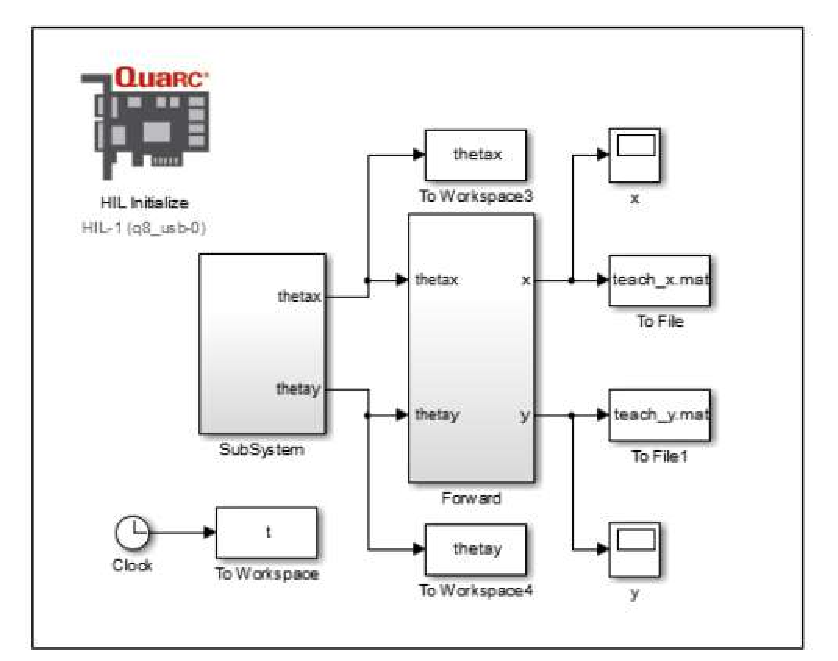
\includegraphics[width=\linewidth]{figure/ex_robot_teach.pdf}
        \caption{実機実験モデル ``ex\_robot\_teach.slx''}
    \end{subfigure}
    \begin{subfigure}[b]{0.48\linewidth}
        \centering
        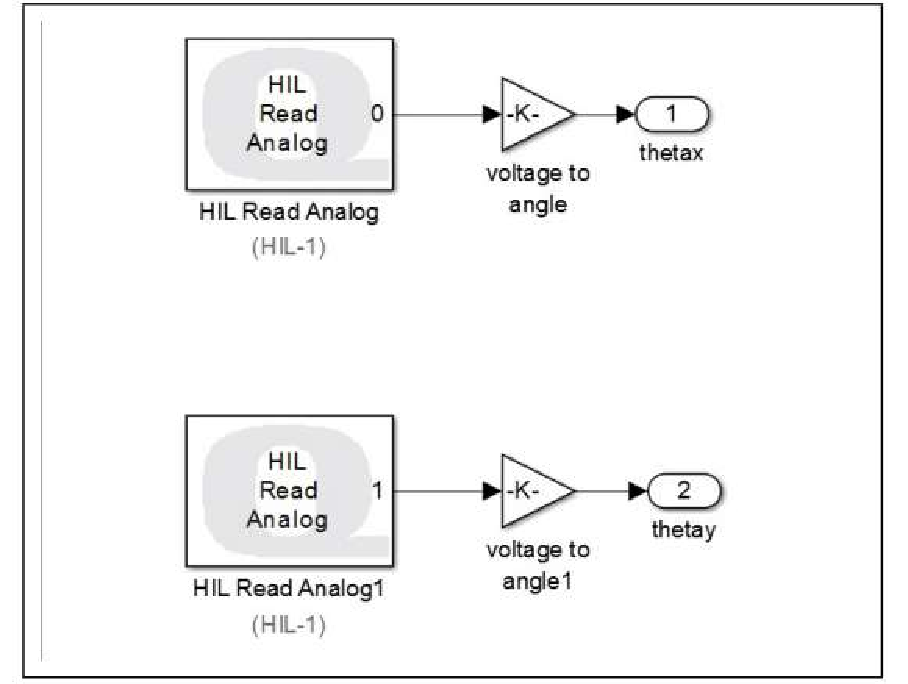
\includegraphics[width=\linewidth]{figure/ex_robot_teach_subsystem.pdf}
        \caption{Subsystem ``2D Robot'' の内容}
    \end{subfigure}
    \caption{教師データ取得のための実機実験モデル ``ex\_robot\_teach.slx''}
    \label{fig:ex_robot_teach}
\end{figure}

つぎに,“\texttt{ex\_robot\_teach.slx}” はデータ取得は30秒間であることに注意し,“Start” アイコンをクリックした後,所望の軌道に沿うように手先を動かす.実験終了後,プロットされたデータが “\texttt{teach\_x.mat}”, “\texttt{teach\_y.mat}” という名前で \texttt{\textbackslash teach} に保存されていることを確認する.

以上の作業が終了した後,\textbf{MATLAB Command Window} で

\begin{lstlisting}[language=Matlab]
load teach_x;
load teach_y;
x_ref_data = teach_x(2,:);    % x_ref の取得
y_ref_data = teach_y(2,:);    % y_ref の取得
t_data     = teach_x(1,:);    

figure(1); plot(t_data,x_ref_data,t_data,y_ref_data);
xlabel('time [s]'); ylabel('{¥it y}^{ref} [m] and {¥it x}^{ref} [m]');

figure(2); plot(x_ref_data,y_ref_data);
xlabel('{¥it x}^{ref} [m]'); ylabel('{¥it y}^{ref} [m]');
\end{lstlisting}

のように入力すると,取得された教師データが図\ref{fig:teaching_data}のように表示される.

\begin{figure}[H]
    \centering
    \begin{subfigure}[b]{0.45\linewidth}
        \centering
        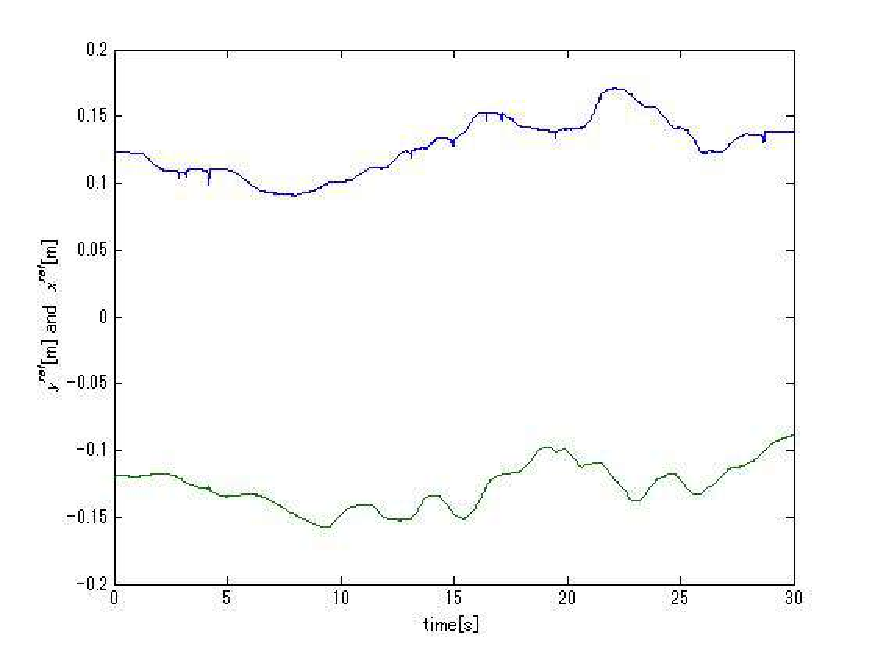
\includegraphics[width=\linewidth]{figure/fig1_xref_yref.pdf}
        \caption{$x^{\mathrm{ref}}(t),\ y^{\mathrm{ref}}(t)$}
    \end{subfigure}
    \begin{subfigure}[b]{0.45\linewidth}
        \centering
        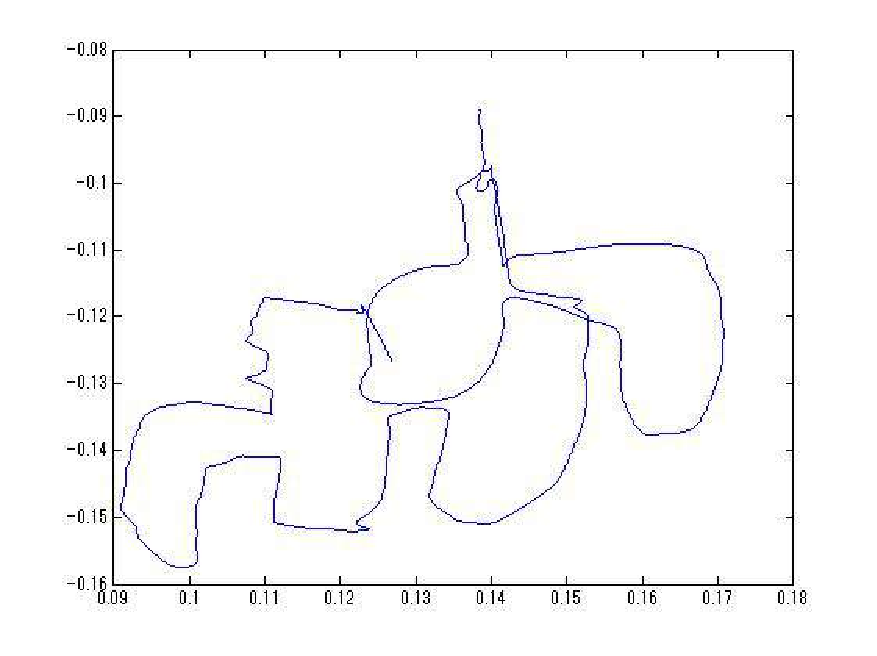
\includegraphics[width=\linewidth]{figure/dairekuto1.pdf}
        \caption{$x$--$y$ 平面での表示}
    \end{subfigure}
    \caption{取得された教師データ}
    \label{fig:teaching_data}
\end{figure}

\subsubsection{シミュレーションと実験}
ステップ1で取得した教師データを目標値($x^{\mathrm{ref}}, y^{\mathrm{ref}}$)として “\texttt{sim\_robot\_xy2.slx}” によりシミュレーションを行い,以下のように入力してシミュレーション結果をアニメーション表示する.

\begin{lstlisting}[language=Matlab]
sim_anime;
\end{lstlisting}

アニメーションにより各リンクに無理な動きがないことを確認した後,“\texttt{ex\_robot\_xy2.slx}” をコンパイルして実機実験を行う.

\subsection{実験結果}
図~\ref{fig:direct_teaching_anim} に示すように,シミュレーション結果のアニメーション表示では,手先が所望の軌道に沿って動いていることが確認できた.また,図~\ref{fig:direct_teaching_result} に示すように,実機実験でも同様の結果が得られた.

\begin{figure}[H]
    \centering
    \begin{subfigure}[b]{0.45\linewidth}
        \centering
        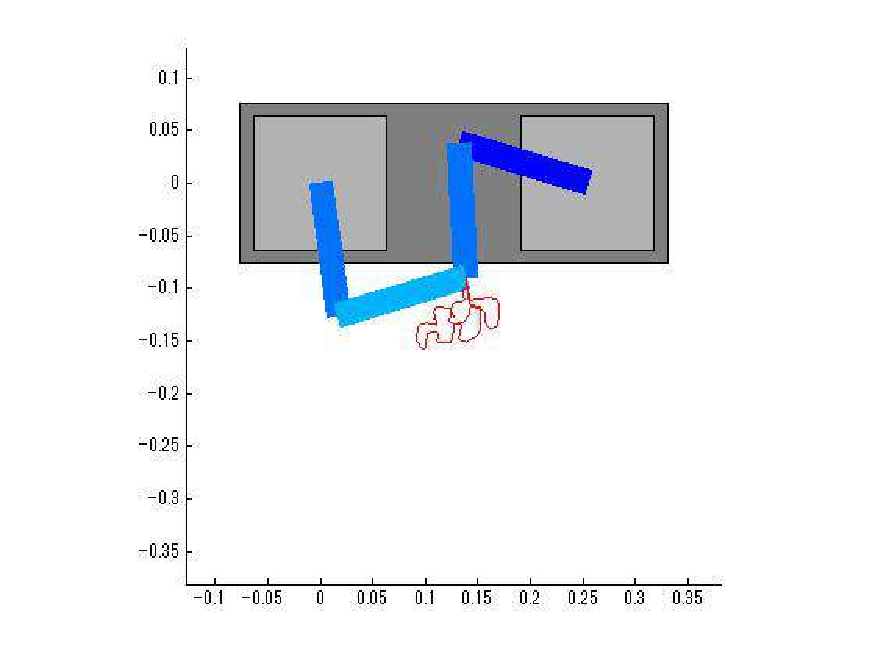
\includegraphics[width=\linewidth]{figure/dairekuto_anime.pdf}
        \caption{シミュレーション結果のアニメーション表示}
        \label{fig:direct_teaching_anim}
    \end{subfigure}
    \begin{subfigure}[b]{0.45\linewidth}
        \centering
        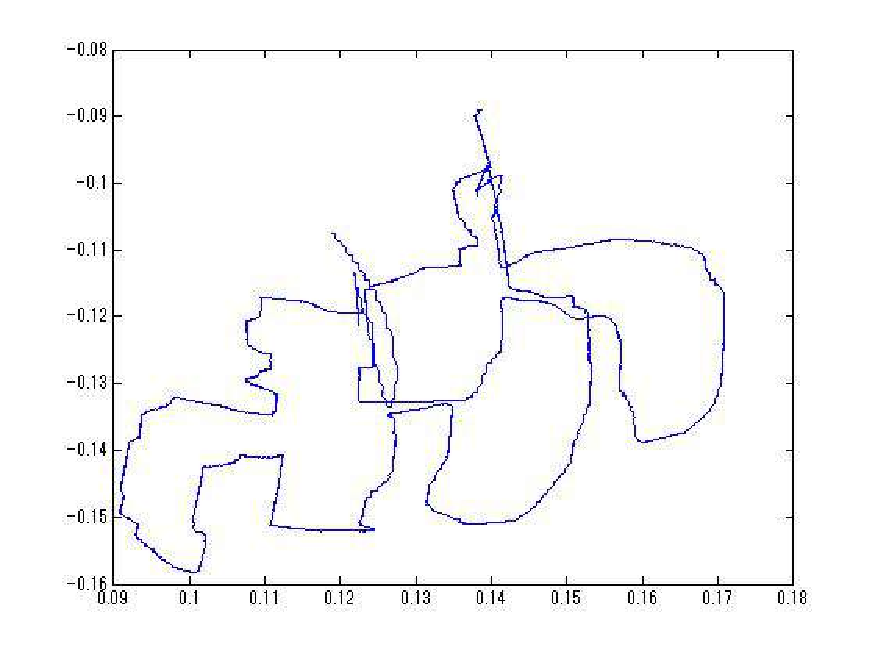
\includegraphics[width=\linewidth]{figure/ex_kekka.pdf}
        \caption{ダイレクトティーチングの実験結果}
        \label{fig:direct_teaching_result}
    \end{subfigure}
    \caption{ダイレクトティーチングにおけるアニメーションと実験結果}
\end{figure}

\subsection{考察}
ダイレクトティーチングでは,手動で動かした手先の軌道を正確に再現できることが確認された.シミュレーションと実機実験の結果が一致しており,制御モデルが正確であることが示された.

ただし,実機実験ではセンサの観測データに若干のノイズが含まれていることが確認された.
このノイズはモーターの不感帯や外部環境の影響によるものであると考えられる.
